\documentclass{article}
\usepackage[utf8]{inputenc}
\usepackage[margin=0.5in]{geometry}
\usepackage{graphicx}
\usepackage{amsmath}
\usepackage{ dsfont }

\graphicspath{ {../figs/} }


\title{Problem Set 3: Quantitative Economics (ECON 8185-001)}
\author{Teerat Wongrattanapiboon}
\date{\today}

\begin{document}
 
 	\maketitle
	
	\noindent\textbf{\Large State Space System} \\
	
	Assume that we have the following state space system:
	
	\begin{align}
		y_t = Z\alpha_t + \epsilon_t \\
		\alpha_t = T \alpha_{t-1} + \eta_t,
	\end{align}
	
	where $\epsilon_t$, $\eta_t$ are assumed to be mean $0$ white noise. Specifically,
	\begin{gather*}
		\mathds{E}[\epsilon_t] =0, \mathds{E}[\eta_t] =0, \mathds{E}[\epsilon_t \eta_s]=0\\
		\mathds{E}[\epsilon_t \epsilon_t'] = H \\
		\mathds{E}[\eta_t \eta_t'] = Q.
	\end{gather*}
 	
	The variables in $y_{t}$ are observed and will be used to construct estimates, while the variables in $\alpha_{t}$ are unobserved and need to be estimated. Equation (1) is the \textbf{measurement} or observer equation and equation (2) is the \textbf{transition} equation for the unobserved state vector. \\
	
	The first step here is to convert a model of interest into a state-space representation. Once we have done that, the \textbf{Kalman Filter} is a system of two equations, the \textbf{predicting} equation and the \textbf{updating} equation. That is,
	\begin{align}
		\hat{\alpha}_{t|t-1} = T \hat{\alpha}_{t-1}\\
		\hat{\alpha}_{t+1|t} = T \hat{\alpha}_{t|t-1} + K_t v_t \\
		y_t = \underbrace{Z \hat{\alpha}_{t|t-1}}_{\hat{y}_{t|t-1}} + v_t
	\end{align}  	
	
	where $\hat{\alpha}_{t|t-1}$ is an estimate of unobserved state vector. The matrix $K_t$ is \textbf{Kalman gain}, and $v_t = y_t - \hat{y}_{t|t-1} = y_t - Z \hat{\alpha}_{t|t-1} $ is an \textbf{innovation}, which is the difference between the observable and its prediction. Note that the prediction of $y_{t}$ (i.e. $\hat{y}_{t|t-1}$) is entirely based on the prediction of state $\hat{\alpha_{t|t-1}}$ as $\hat{y}_{t|t-1} = Z\hat{\alpha_{t|t-1}}$. Hence, Kalman Filter evolves around predicting $\hat{\alpha}_{t|t-1}$ and updating the prediction of the state vector $\hat{\alpha}_{t+1|t}$. \\
	
	At time $t$, before we have actually observed $y_t$, our information set consists of lagged values of $y: (y_0, y_1, \dots, y_{t-1}).$ Based on this information, we begin by making the best guess for the underlying state. From the law of motion of state we have:
	\begin{align*}
		\hat{\alpha}_{t|t-1} = \mathds{E}[\alpha_t | (y_0, y_1, \dots, y_{t-1}) ] = T\mathds{E}[\alpha_{t-1}|(y_0, y_1, \dots, y_{t-1})] + 				\underbrace{\mathds{E}[\eta_t|(y_0, y_1, \dots, y_{t-1})]}_{0}.
	\end{align*}
	Define $\hat{\alpha}_{t-1} = \mathds{E}[\alpha_{t-1}| y_0, y_1, \dots , y_{t-1}]$. We can then write $\hat{\alpha}_{t|t-1} = T\hat{\alpha}_{t-1}$, which is a function of lagged values of $y$. At time $t$, we also have the variance of prediction error as:
	\begin{align*}
		P_{t-1} = \mathds{E}[(\alpha_{t-1} - \hat{\alpha}_{t-1})(\alpha_{t-1} - \hat{\alpha}_{t-1})'].
	\end{align*}
	
	The conditional variance of prediction error is given by:
	\begin{align*}
		P_{t|t-1} &  = \mathds{E}[(\alpha_t - \hat{\alpha}_{t|t-1})(\alpha_t - \hat{\alpha}_{t|t-1})']\\
		& = \mathds{E}[(T\alpha_{t-1} + \eta_t - T\hat{\alpha}_{t-1})(T\alpha_{t-1} + \eta_t - T\hat{\alpha}_{t-1})']\\
		& = \mathds{E}[(T(\alpha_{t-1}-\hat{\alpha}_{t-1})+ \eta_t)(T(\alpha_{t-1}-\hat{\alpha}_{t-1})+ \eta_t)'] \\
		& = T\mathds{E}[(\alpha_{t-1}-\hat{\alpha}_{t-1})(\alpha_{t-1}-\hat{\alpha}_{t-1})']T'+ \mathds{E}[\eta_t\eta_t']\\
		& = TP_{t-1}T' + Q,
	\end{align*}
	which follows from the fact that $(\alpha_{t-1}-\hat{\alpha}_{t-1})$ and $\eta_t$ are uncorrelated. The conditional variance of the innovation is given by: 
	\begin{align*}
		F_t & = \mathds{E}[v_t v_t'] \\
		& = \mathds{E}[(y_t - Z \hat{\alpha}_{t|t-1})(y_t - Z \hat{\alpha}_{t|t-1})']\\
		& = \mathds{E}[(Z \alpha_t - Z \hat{\alpha}_{t|t-1})( Z \alpha_t - Z \hat{\alpha}_{t|t-1})']\\
		& = Z P_{t|t-1}Z' + H,
	\end{align*}
	and the covariance of $v_t$ with the estimation error is:
	\begin{align*}
		G_t & = \mathds{E}[(y_t - \hat{y}_{t|t-1})(\alpha_t - \hat{\alpha}_{t|t-1})']\\
		& = \mathds{E}[(Z\alpha_t - Z\hat{\alpha}_{t|t-1} + \epsilon_t)(\alpha_t - \hat{\alpha}_{t|t-1})'] \\
		& = ZP_{t|t-1}.
	\end{align*}
	Note that before we actually observe $y_t$, conditional on the information set $(y_0, y_1, \dots, y_{t-1})$, all the matrices $P_{t-1}, P_{t|t-1}, F_t, G_t$, are known. \\

	For jointly Normal random variable $X$ and $Y$ with the variance-covariance matrix given by:
	\begin{align*}
		\Sigma = \begin{bmatrix}
		\Sigma_{XX} & \Sigma_{XY} \\
		\Sigma_{XY} & \Sigma_{YY}
		\end{bmatrix},
	\end{align*}
	
	and the conditional expectation of $Y$ given $X$ is given by:
	\begin{align*}
		\mathds{E}[Y|X] = \mathds{E}[Y] + \Sigma_{XY} \Sigma_{XX}^{-1}(X - \mathds{E}[X]),
	\end{align*}
	
	and the conditional variance is given by:
	\begin{align*}
		Var[Y|X] = \mathds{E}[(Y - E[Y|X])^2] = \Sigma_{YY} - \Sigma_{YX}\Sigma_{XX}^{-1}\Sigma_{XY}.
	\end{align*}
	
	It then follows from the above formula that:
	$$
		\mathds{E}[\alpha_t| (y_0, y_1, \dots, y_{t-1}), y_t]=\mathds{E}[\alpha_t|(y_0, y_1, \dots, y_{t-1})] + Cov(\alpha_t, y_t)Var(y_t)^{-1}(y_t - \mathds{E}[y_t | (y_0, y_1, \dots, y_{t-1})]).
	$$
	\begin{align*}
		Cov(\alpha_t, y_t ) &  = \mathds{E}[(\alpha_t - E[\alpha_t|(y_0, y_1, \dots, y_{t-1})])(y_t - E[y_t | (y_0, y_1, \dots, y_{t-1})])']\\
		& = \mathds{E}[(\alpha_t - \hat{\alpha}_{t|t-1})(y_t - \hat{y}_{t|t-1})']\\
		& = P_{t|t-1}Z' \\
		Var(y_t) & = \mathds{E}[(y_t - E[y_t|(y_0, y_1, \dots, y_{t-1})])(y_t - E[y_t|(y_0, y_1, \dots, y_{t-1})']\\
		& = \mathds{E}[(y_t - \hat{y}_{t|t-1})(y_t - \hat{y}_{t|t-1} )']\\
		& = ZP_{t|t-1}Z' + H.
	\end{align*}
	
	Hence, the updating equation is given by:
	\begin{align*}
		\hat{\alpha}_t & = \hat{\alpha}_{t|t-1} + P_{t|t-1}Z'(ZP_{t|t-1}Z' + H)^{-1}(y_t - \hat{y}_{t|t-1})\\
		& =  \hat{\alpha}_{t|t-1} + G_t' F_t^{-1}(y_t - \hat{y}_{t|t-1}).
	\end{align*}
	
	Multiplying both sides of previous equation by T we get:
	\begin{align*}
		\hat{\alpha}_{t+1|t} = T\hat{\alpha}_{t|t-1} + K v_t
	\end{align*}
	
	where $K = TP_{t|t-1}Z'(ZP_{t|t-1}Z' + H)^{-1} = T G_t' F_t^{-1}$, and $v_t = y_t - \hat{y}_{t|t-1}$. Similarly, using the conditional variance formula, we obtain
	\begin{align*}
		P_t = P_{t|t-1} - G_t'F_t^{-1}G_t.
	\end{align*}
	
	\noindent\textbf{\Large Kalman Filter} \\
	
	\begin{enumerate}
		\item Begin with a guess for $\alpha_0$, $P_0$.  We can set $\alpha_0$ to be the unconditional mean of state vector, and $P_0$ to be the stationary $P$ that solves $P = TPT' + Q$. Set $\hat{\alpha}_{1|0} = T \alpha_0$, and  $P_{1|0} = TP_{0}T' + Q$.
		\item Compute:
		\begin{enumerate}
			\item $\hat{y}_{1|0} = Z\hat{\alpha}_{1|0}$
			\item $v_1 = y_1 - \hat{y}_{1|0} $
			\item $F_1 = ZP_{1|0}Z' + H, G_1 = ZP_{1|0}, K_1 = TG_1'F_1^{-1}$
			\item $\hat{\alpha}_{2|1} = T \hat{\alpha}_{1|0} + K_1 v_1$
			\item $P_{2|1} = T(P_{1|0} - G_1'F_1^{-1}G_1)T' + Q$
			\item Go back to step $(a)$ increasing the time order by $1$ unit.
		\end{enumerate}
		\item Continue the recursion in this fashion to get sequence of $\{ \hat{\alpha}_{t|t-1} \}$, $\{i_t\}$ and $\{\hat{y}_{t|t-1}\}.$
	\end{enumerate}

	\noindent\textbf{\Large Parametric Estimation using Log Likelihood} \\
	
	To compute parameters, we maximize the following log-likelihood:
	\begin{align*}
		\ln L = \sum_t \left\{ -\frac{n}{2} \ln 2\pi -\frac{1}{2}\ln |F_t| - \frac{1}{2}v_t'F_t^{-1}v_t \right\}. 
	\end{align*}
	
	\noindent\textbf{\Large Question 1} \\
	
	First, let's write each process in state space representation.
	
	\begin{enumerate}
		\item $\text{AR}(1): x_t = \rho x_{t-1} + \epsilon_t$ \\
			\textbf{State}: \hspace{4mm} $x_t = [\rho]x_{t-1} + \epsilon_t$ \\
			\textbf{Observation}: $ x_t = [1]x_t$
		\item $\text{AR}(2): x_t = \rho_1 x_{t-1} + \rho_2 x_{t-2} + \epsilon_t$\\
			\textbf{State}: \hspace{4mm} $\begin{bmatrix} x_t \\ x_{t-1} \end{bmatrix} = \begin{bmatrix} \rho_1 & \rho_2 \\ 1 & 0\end{bmatrix}\begin{bmatrix} x_{t-1} \\ x_{t-2} \end{bmatrix} + \begin{bmatrix} 1 \\ 0 \end{bmatrix} \epsilon_t $ \\
			\textbf{Observation}: $ x_t = \begin{bmatrix} 1 & 0\end{bmatrix} \begin{bmatrix}x_t \\ x_{t-1}\end{bmatrix}$

		\item $\text{MA}(1): x_t = \epsilon_t + \rho \epsilon_{t-1}$\\

			\textbf{State}: \hspace{4mm} $\begin{bmatrix} \epsilon_t \\ \epsilon_{t-1} \end{bmatrix} = \begin{bmatrix} 0 & 0 \\ 1 & 0 \end{bmatrix}
\begin{bmatrix} \epsilon_{t-1} \\ \epsilon_{t-2} \end{bmatrix} + \begin{bmatrix} 1 \\ 0 \end{bmatrix} \epsilon_t $ \\
			\textbf{Observation}: $ x_t = \begin{bmatrix} 1 & \rho \end{bmatrix} \begin{bmatrix}\epsilon_t \\ \epsilon_{t-1}\end{bmatrix}$

		\item $\text{Random Walk}: x_{t} = \mu_{t} + \epsilon_{t}$, $\mu_{t} = \mu_{t-1} + \eta_{t}$

			\textbf{State}: \hspace{4mm} $\mu_t = [1]\mu_{t-1} + \eta_t$ \\
			\textbf{Observation}: $x_t = [1]\mu_t + \epsilon_t.$

	\end{enumerate}
	
	\newpage
	
	\noindent\textbf{\Large Results} \\
	
	\noindent\textbf{\large AR(1)} \\
	
	We set $\rho = 0.6$ and $\sigma = 0.5$, simulate the AR(1) process for $100$ periods, and apply the Kalman filter algorithm to obtain the following plot:
	
	\begin{figure}[htbp]
		\centering
		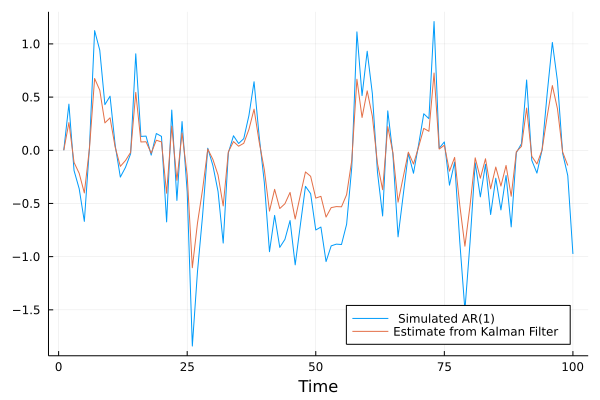
\includegraphics[scale=0.5]{AR1.png}
		\caption{Simulated and Filtered AR(1)}
	\end{figure} 
	
	We then use the log-likelihood function given above to compute the likelihood of observing this simulated process, and maximize the likelihood with respect to the AR(1) parameters to obtain their best estimates. The estimated parameters are $\hat{\rho} = 0.61$ and $\hat{\sigma} = 0.48$, which are pretty close to the actual parameters. \\
	
	\noindent\textbf{\large AR(2)} \\
	
	We set $\rho_{1} = 0.3$, $\rho_{2} = 0.4$, $\sigma = 0.5$, simulate the AR(2) process for $100$ periods, and apply the Kalman filter algorithm to obtain the following plot:
	
	\begin{figure}[htbp]
		\centering
		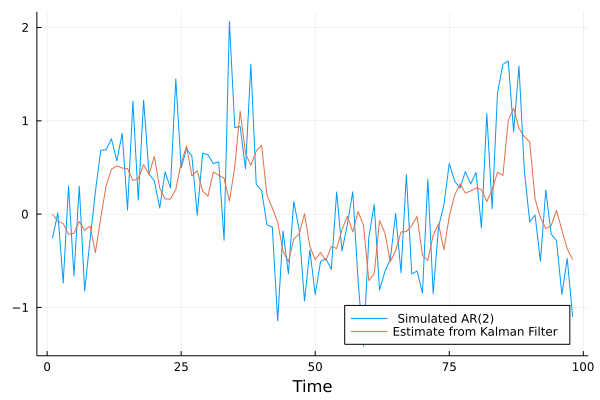
\includegraphics[scale=0.5]{AR2.png}
		\caption{Simulated and Filtered AR(2)}
	\end{figure} 
	
	The estimated parameters are $\hat{\rho}_{1} = 0.26$ and $\hat{\rho}_{2} = 0.48$, and $\hat{\sigma} = 0.54$. \\
	
	\noindent\textbf{\large MA(1)} \\
	
	We set $\rho = 0.7$, $\sigma = 0.8$, simulate the MA(1) process for $100$ periods, and apply the Kalman filter algorithm to obtain the following plot:
	
	\begin{figure}[htbp]
		\centering
		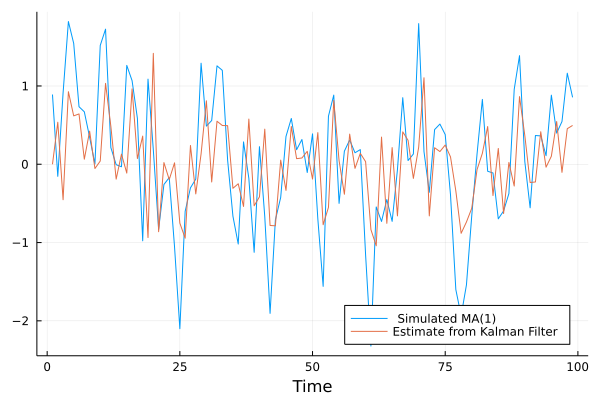
\includegraphics[scale=0.5]{MA1.png}
		\caption{Simulated and Filtered MA(1)}
	\end{figure} 
	
	The estimated parameters are $\hat{\rho} = 0.61$ and $\hat{\sigma} = 0.73$. \\
	
	\noindent\textbf{\large Random Walk} \\
	
	We set $\sigma_{\epsilon} = 0.8$, $\sigma_\eta = 0.6$, simulate the random walk process for $100$ periods, and apply the Kalman filter algorithm to obtain the following plot:
	
	\begin{figure}[htbp]
		\centering
		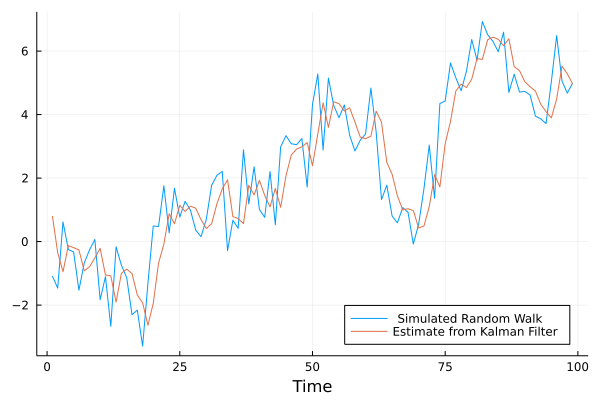
\includegraphics[scale=0.5]{RW.png}
		\caption{Simulated and Filtered Random Walk}
	\end{figure} 
	
	The estimated parameters are $\hat{\sigma}_{\epsilon} = 0.70$ and $\hat{\sigma}_{\eta} = 0.65$. \\
 	
\end{document}